\begin{slide}{Back Propagation in TensorFlow}
  \centering
    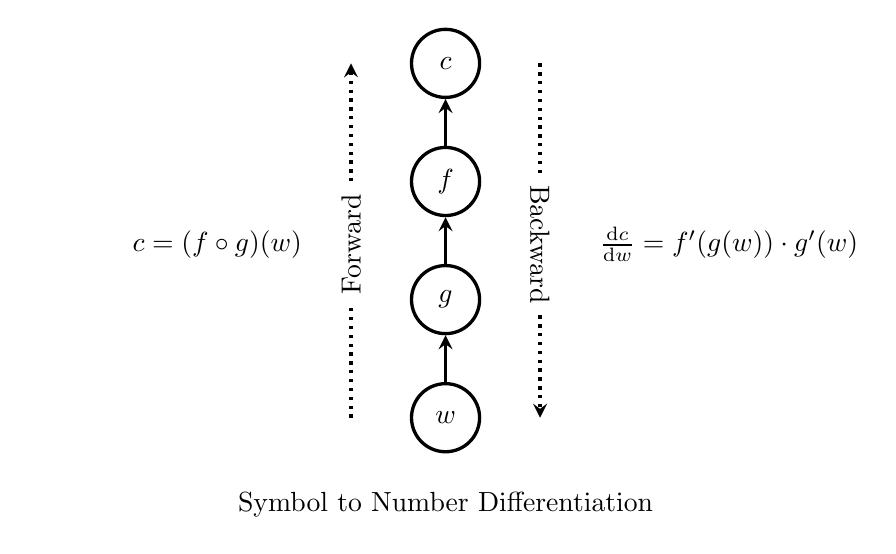
\begin{tikzpicture}
      \onslide<2->{
     % Nodes
      \path [very thick] (0, 0)
            coordinate [draw, circle, text width=0.6cm] (w) node {$w$};
      \path [very thick] (0, 1.5)
             coordinate [draw, circle, text width=0.6cm] (g) node {$g$};
      \path [very thick] (0, 3)
            coordinate [draw, circle, text width=0.6cm] (f) node {$f$};
      \path [very thick] (0, 4.5)
            coordinate [draw, circle, text width=0.6cm] (c) node {$c$};

      % Edges
      \draw [very thick, -stealth] (w) -- (g);
      \draw [very thick, -stealth] (g) -- (f);
      \draw [very thick, -stealth] (f) -- (c);
      }

      % Label
     \onslide<3->{
        \draw (0, -1.1) node {Symbol to Number Differentiation};
      }

    \onslide<4->{
      % Forward Propagation
      \draw [very thick, -stealth, dotted]
            (-1.2, 0) -- +(0, 1.4)
            (-1.2, 3) -- +(0, 1.5);
      \draw (-1.2, 2.2) node [rotate=90] {Forward};
      \draw (-1.4, 2.2) node [left] {$c = (f \circ g)(w)\hspace{0.3cm}$};

      % Spacing
      \draw (4.2, 0);
    }

    \onslide<5->{
      % Backward Propagation
      \draw [very thick, -stealth, dotted]
            (+1.2, 4.5) -- +(0, -1.4)
            (+1.2, 1.3) -- +(0, -1.3);
      \draw (+1.2, 2.2) node [rotate=270] {Backward};
      \draw (+3.6, 2.2) node {$\frac{\mathrm{d}c}{\mathrm{d}w} = f'(g(w)) \cdot g'(w)$};

     % Spacing
     \draw (-5.3, 0);
    }
  \end{tikzpicture}
\end{slide}

\begin{slide}{Back Propagation in TensorFlow}
  \centering
    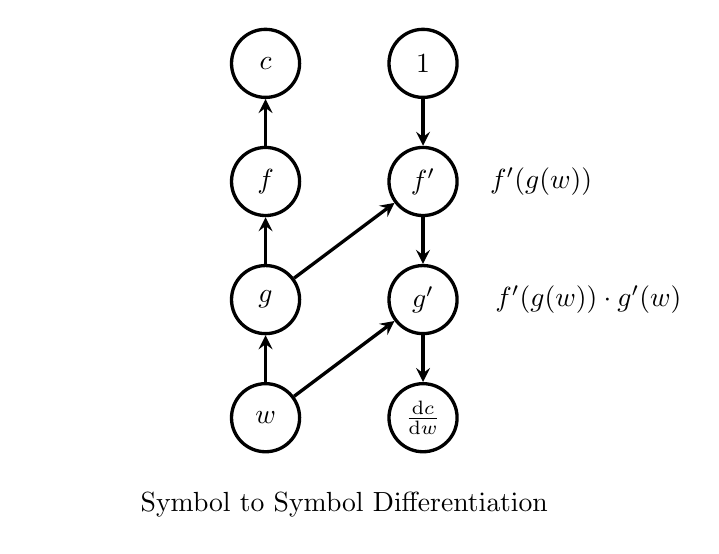
\begin{tikzpicture}[very thick]
     % Nodes
      \path [very thick] (0, 0)
            coordinate [draw, circle, text width=0.6cm] (w) node {$w$};
      \path [very thick] (0, 1.5)
             coordinate [draw, circle, text width=0.6cm] (g) node {$g$};
      \path [very thick] (0, 3)
            coordinate [draw, circle, text width=0.6cm] (f) node {$f$};
      \path [very thick] (0, 4.5)
            coordinate [draw, circle, text width=0.6cm] (c) node {$c$};

      % Edges
      \draw [very thick, -stealth] (w) -- (g);
      \draw [very thick, -stealth] (g) -- (f);
      \draw [very thick, -stealth] (f) -- (c);

      % Label
     \draw (1, -1.1) node {Symbol to Symbol Differentiation};

     \onslide<2->{
       % Gradient Nodes
       \path [very thick] (2, 4.5)
             coordinate [draw, circle, text width=0.6cm] (dc) node {$1$};
     }

     \onslide<3->{
       % Gradient Nodes
       \path (2, 3) coordinate [draw, circle, text width=0.6cm] (df) node {$f'$};

       % Gradient Edges
       \draw [-stealth] (dc) -- (df);
       \draw [-stealth] (g) -- (df);

       % Gradient Labels
       \draw (3.5, 3) node {$f'(g(w))$};
     }

     \onslide<4->{
       \path (2, 1.5) coordinate [draw, circle, text width=0.6cm] (dg) node {$g'$};

       % Gradient Edges
       \draw [-stealth] (df) -- (dg);
       \draw [-stealth] (w) -- (dg);

       % Gradient Labels
       \draw (4.1, 1.5) node {$f'(g(w)) \cdot g'(w)$};
     }

     \onslide<5->{
       \path (2, 0) coordinate [draw, circle, text width=0.6cm]
            (dw) node {$\frac{\mathrm{d}c}{\mathrm{d}w}$};

       % Gradient Edges
       \draw [-stealth] (dg) -- (dw);
     }

     % Spacing
     \draw (-3, 0);
  \end{tikzpicture}
\end{slide}

%%% Local Variables:
%%% mode: latex
%%% TeX-master: "../presentation.tex"
%%% End:
